\chapter{Listas con empates}

Retomemos el problema planteado en el capítulo \ref{me}, recordemos que se planteo el problema del matrimonio estable y se demostro que sin importar si las listas de preferencia son completas o incompletas, existe un algoritmo polinomial que siempre encuentra un emparejamiento estable optimo (en el sentido de los hombres o de las mujeres dependendiendo de que algoritmo se use). \\

Ahora, consideremos el caso en el que la lista de preferencias es completo, es decir cada hombre y cada mujer tiene catalogado en su orden de preferencia a cada persona del genero opuesto. Incluiremos la variante de que en la lista se pueden introducir empates, esto es muy común dada que en muchas ocasiones la diferencia entre escoger a dos personas puede ser no significativa. 

\begin{eje}{\cite{Verde}}
\label{ejemplo empates}
Supongamos que para 2 hombres y 2 mujeres tenemos la matriz de preferencias 
$$\begin{pmatrix}
& A & B  \\
\alpha & 1,2 & 2,2 \\
\beta & 1,1 & 1,1\\
\end{pmatrix}.$$

En este caso el orden de preferencias $A$ y $B$ es $(\beta, \alpha)$, el orden de preferencia de $\alpha$ es $(A,B)$ y el orden de preferencia de $\beta$ es $([A,B])$\footnote{los corchetes denotan que la lista contiene empates}.
\end{eje}

Para este caso es necesario cambiar un poco la definición de estabilidad y de inestabilidad. 

\begin{dfn}{\cite{Verde}}
\label{estricto}
Decimos que un emparejamiento es inestable si existen un hombre $\alpha$ y una mujer $\beta$, donde cada uno de ellos \textbf{estrictamente} prefiere al otro que a su respesctiva pareja.  \\
Alternativamente un emparejamiento es estable si no es inestable.
\end{dfn}

La unica diferencia con la definición \ref{Estable} es la palabra estrictamente, este tipo de emparejamientos en muchas ocasiones se conoce como \textbf{estabilidad debil}\footnote{Si no se pide la preferencia estricta es posible ver que en muchas ocasiones no existe un emparejamiento estable para el problema (ver \cite{Verde}).}. En el caso de que no existan empates en las listas de preferencias las dos definciones son identicas. El siguiente resultado muestra que el algoritmo de Gale Shapley tambien sirve para encontrar un emparejamiento estable dadas estas condiciones.

\begin{cor}
Dada una matriz de preferencias arbitaria completa en la que se permiten empates con $n$ hombres y $m$ mujeres, el algoritmo de Gale Shapley converge a un emparejamiento estable.
\end{cor}
\begin{proof}
De la definición \ref{estricto} podemos ver que si partimos si convertimos los empates en ordenes estrictos de forma arbitraria llegamos a una instancia del problema planteado en el capítulo \ref{me}. Si aplicamos el resultado del teorema \ref{teorema de Gale Shapley} podemos ver que el algoritmo converge a un emparejamiento estable.  \\
\end{proof}

Una nota importante de la demostración de arriba es que si que si cambiamos los empates en ordenes distrintos podríamos llegar a emparejamientos estables diferentes. 





\begin{eje}
Consideremos la lista de preferencias del ejemplo \ref{ejemplo empates}, la modificamos para que permita un orden estricto obteniendo la siguiente matriz de preferencias
$$\begin{pmatrix}
& A & B  \\
\alpha & 1,2 & 2,2 \\
\beta & 1,1 & 2,1\\
\end{pmatrix}.$$
En primera instancia, $\alpha$ y $\beta$ le proponen a $A$.

\begin{figure}[H]
\centering

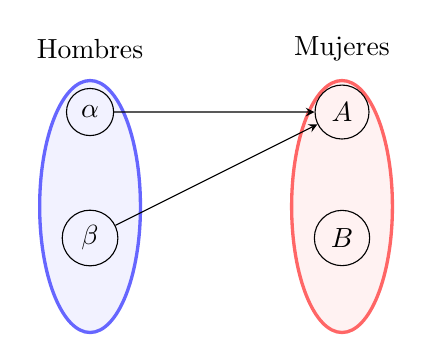
\begin{tikzpicture}[ scale=0.8]
\tikzset{vertex/.style = {shape=circle,draw,minimum size=1.5em}}
\tikzset{edge/.style = {->,> = latex}}
\filldraw[color=blue!60, fill=blue!5, very thick](0,2.5) ellipse (.8 and 2);
\filldraw[color=red!60, fill=red!5, very thick](4,2.5) ellipse (.8 and 2);


% vertices
% 


\node[vertex] (a) at (0,4) {$\alpha$};
\node[vertex] (b) at (0,2) {$\beta$};


\node[vertex] (e) at (4,4) {$A$};
\node[vertex] (f) at (4,2) {$B$};

%\draw (0,.5) node[cross,red] {};

\node (i) at (0,5) {Hombres};
\node (j) at (4,5) {Mujeres};

\path[-stealth] (a) edge (e);
\path[-stealth] (b) edge (e);




%\draw (0.2,8)--(3.8,8);



\end{tikzpicture}

\caption{Primera iteración.}
\end{figure}
En segunda instancia, $A$ acepta la propuesta de $\beta$ y $\alpha$ le propone matrimonio a $B$.

\begin{figure}[H]
\centering

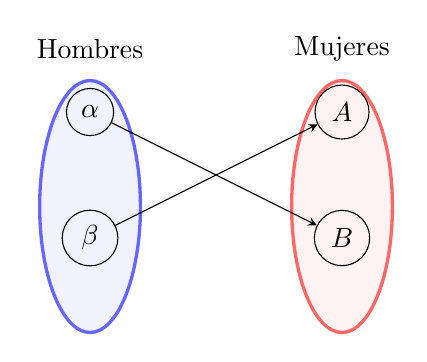
\begin{tikzpicture}[ scale=0.8]
\tikzset{vertex/.style = {shape=circle,draw,minimum size=1.5em}}
\tikzset{edge/.style = {->,> = latex}}
\filldraw[color=blue!60, fill=blue!5, very thick](0,2.5) ellipse (.8 and 2);
\filldraw[color=red!60, fill=red!5, very thick](4,2.5) ellipse (.8 and 2);


% vertices
% 


\node[vertex] (a) at (0,4) {$\alpha$};
\node[vertex] (b) at (0,2) {$\beta$};


\node[vertex] (e) at (4,4) {$A$};
\node[vertex] (f) at (4,2) {$B$};

%\draw (0,.5) node[cross,red] {};

\node (i) at (0,5) {Hombres};
\node (j) at (4,5) {Mujeres};

\path[-stealth] (a) edge (f);
\path[-stealth] (b) edge (e);




%\draw (0.2,8)--(3.8,8);



\end{tikzpicture}

\caption{Segunda iteración.}
\end{figure}

Es claro que el emparejamiento obtenido despues de dos iteraciones es estable.
\end{eje}

Otro resultado importante de este problema es que sigue cumpliendo el teorema \ref{rural}, es decir dados dos emparejamientos estables la cantidad de hombres emparejados es la misma.

\begin{cor}
Dada una matriz de preferencias completa en la que se permiten empates con $n$ hombres y $m$ mujeres. Si tenemos dos emparejamientos estables $M_1$ y $M_2$, la cantidad de hombres emparejados es la misma.
\end{cor}
\begin{proof}
Dada que la lista de preferencias es completa, todos los hombres prefieren tener a una pareja (sin importar que mujer les toque) a quedarse solos, lo mismo es cierto para las mujeres. Por lo tanto, el número de hombres emparejados es el mínimo entre el número de hombres y el número de mujeres. 
\end{proof}

\section{Listas incompletas con empates}
Ahora, consideremos el problema del matrimonio estable considerando dos variantes para el problema; la lista de preferencias es incompleta, o sea para alguna persona en el problema existe otra persona del genero opuesto de la cual prefiere quedarse no emparejado a terminar emparejado con ella y además se permiten empates en la lista del mismo modo que se planteo al principio del capítulo. 

\begin{eje}{\cite{empates}}
Supongamos que para 2 hombres y 2 mujeres tenemos la matriz de preferencias 
$$\begin{pmatrix}
& A & B  \\
\alpha & 1,1 & , \\
\beta & 1,1 & 2,1\\
\end{pmatrix}.$$
En este caso el orden de preferencias de $\alpha$ es $(A)$, el orden de preferencias de $\beta$ es $(A,B)$, el orden de preferencias de $A$ es $([\alpha,\beta])$ y el orden de preferencias de $B$ es $(\alpha)$. \\
Para este problema existen dos emparejamientos estables:
\begin{figure}[H]
\centering

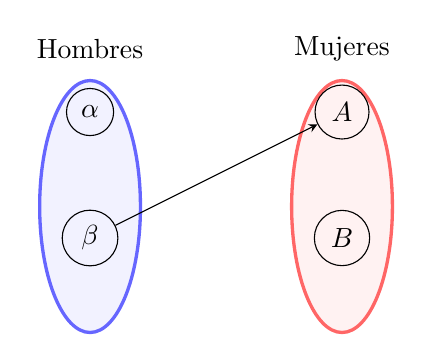
\begin{tikzpicture}[ scale=0.8]
\tikzset{vertex/.style = {shape=circle,draw,minimum size=1.5em}}
\tikzset{edge/.style = {->,> = latex}}
\filldraw[color=blue!60, fill=blue!5, very thick](0,2.5) ellipse (.8 and 2);
\filldraw[color=red!60, fill=red!5, very thick](4,2.5) ellipse (.8 and 2);


% vertices
% 


\node[vertex] (a) at (0,4) {$\alpha$};
\node[vertex] (b) at (0,2) {$\beta$};


\node[vertex] (e) at (4,4) {$A$};
\node[vertex] (f) at (4,2) {$B$};

%\draw (0,.5) node[cross,red] {};

\node (i) at (0,5) {Hombres};
\node (j) at (4,5) {Mujeres};

\path[-stealth] (b) edge (e);
%\path[-stealth] (b) edge (e);




%\draw (0.2,8)--(3.8,8);



\end{tikzpicture}

\caption{Primer emparejamiento estable.}
\end{figure}

\begin{figure}[H]
\centering

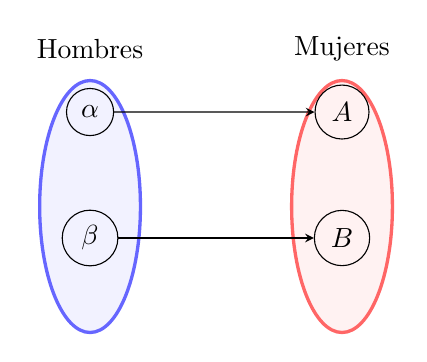
\begin{tikzpicture}[ scale=0.8]
\tikzset{vertex/.style = {shape=circle,draw,minimum size=1.5em}}
\tikzset{edge/.style = {->,> = latex}}
\filldraw[color=blue!60, fill=blue!5, very thick](0,2.5) ellipse (.8 and 2);
\filldraw[color=red!60, fill=red!5, very thick](4,2.5) ellipse (.8 and 2);


% vertices
% 


\node[vertex] (a) at (0,4) {$\alpha$};
\node[vertex] (b) at (0,2) {$\beta$};


\node[vertex] (e) at (4,4) {$A$};
\node[vertex] (f) at (4,2) {$B$};

%\draw (0,.5) node[cross,red] {};

\node (i) at (0,5) {Hombres};
\node (j) at (4,5) {Mujeres};

\path[-stealth] (a) edge (e);
\path[-stealth] (b) edge (f);




%\draw (0.2,8)--(3.8,8);



\end{tikzpicture}

\caption{Segundo emparejamiento estable.}
\end{figure}
\end{eje}

Un resultado directo mostrado en el ejemplo de arriba es el siguiente corolario.

\begin{cor}
Dada una matriz de preferencias incompleta en la que se permiten empates para $n$ hombres y $m$ mujeres. Si tenemos dos emparejamientos estables $M_1$ y $M_2$, la cantidad de hombres emparejados no necesariamente es la misma.
\end{cor}

Un problema interesante aquí es encontrar \textbf{un emparejamiento estable de máxima cardinalidad}, o sea encontrar algun emparejamiento estable $M_1$ con la propiedad de que no existe ningun otro emparejamiento $M_2$ estable en el problema en el cual exista una mayor cantidad de hombres emparejados que en $M_1$.  El siguiente resultado muestra que encontrar una solución para este problema no es nada trivial.

\begin{teo} {\cite{empates}}
Dada una matriz de preferencias incompleta en la que se permiten empates para $n$ hombres y $n$ mujeres. El problema de encontrar un emparejamiento estable de máxima cardinalidad es NP-duro. Este resultado es correcto inclusive si solo existen empates en las listas de las mujeres (o de forma análoga en las listas de los hombres). 
\end{teo}
\begin{proof}
Tomemos $k$ un entero no negativo fijo y consideremos el problema de decisión de encontrar un emparejamiento estable $M$ para el problema anterior con la propiedad de que la cantidad de hombres emparejados en $M$ es mayor o igual que $k$, para facilitar la notación en el problema llamaremos a este problema de notación como \text{Max Cardinality SMTI}\footnote{SMTI quiere decir emparejamientos estables con listas incompletas y empates.}\footnote{Se considera el nombre en ingles para ser consistente con los artículos publicados sobre el tema.}. Claramente si Max Cardinality SMTI esta en NP y además si Max Cardinality SMTI es NP-completo entonces el problema de encontrar un emparejamiento estable de máxima cardinalidad es NP-duro. \\
Para demostrar que este Max Cardinality SMTI es NP-completo, transformamos el problema al de encontrar un emparejamiento estable maximal para gráficas de subdivisión.
% Falta acabar esta demostración. 
\end{proof}














